\subsection{OB-12 (ASB)}
Kryptografické síťové protokoly, využití šifrování a algoritmu Diffie-Hellman. Protokoly TLS a SSH.

\subsubsection*{Šifrování na různých vrstvách}
\begin{itemize}
	\item šifrování na vrstvě $x$ znamená ukrytí dat vrstvy $x+1$
	\item aplikační vrstva --- šifrování řeší aplikace sama, šifrování jsou různá, závislá na aplikaci
	\item transportní vrstva --- SSL/TLS, ukrývá data a protokol aplikace
	\item síťová vrstva --- některé VPN, IPsec --- ukrývá data transportní vrstvy
	\item linková vrstva --- Wi-Fi
\end{itemize}

\subsubsection*{TLS}
\begin{itemize}
	\item šifrování na transportní vrstvě
	\item TLS se skládá z následujících vrstev:
	
	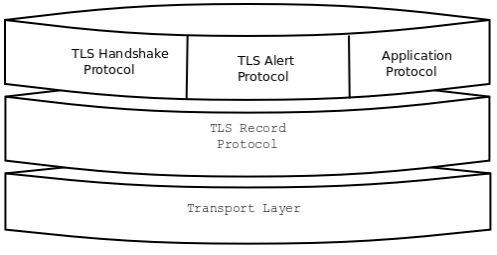
\includegraphics[width=0.6\textwidth]{img/OB-12_0.jpg}
	
	\item Record Layer --- vrstva zodpovědná za posílání TLS zpráv, skládá se z z dalších vrstev
	\item Handshake Protocol --- výběr šifrovací sady, parametrů spojení a ustanovení společných klíčů
	\item Alert Protocol --- přenos chybových zpráv, např. neplatný certifikát
	\item Application Protocol --- šifrovaný protokol aplikační vrstvy
	\item TLS handshake:
	
	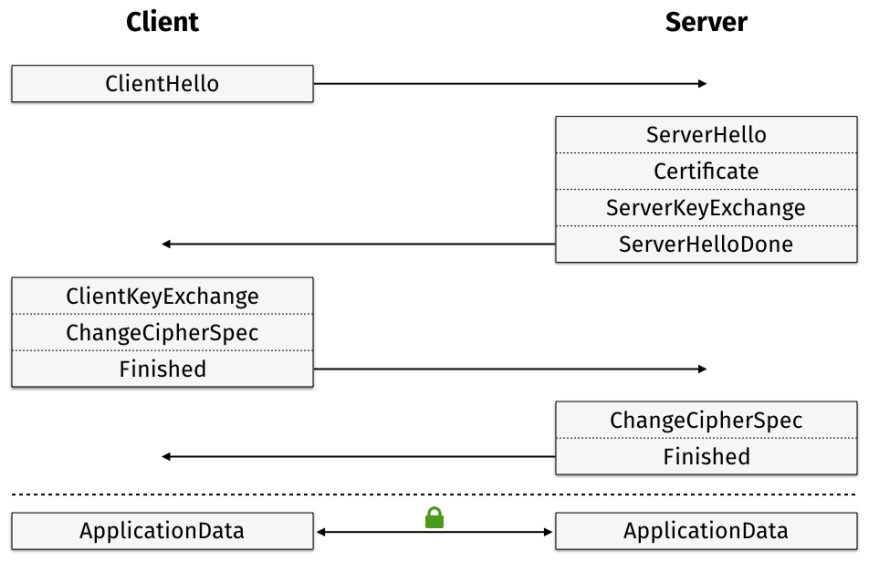
\includegraphics[width=0.8\textwidth]{img/OB-12_1.jpg}
	
	\begin{itemize}
		\item Client Hello --- obsahuje aktuální (UNIXový) čas, náhodné číslo (28B), podporované šifrovací sady a rozšíření
		\item Server Hello --- obsahuje aktuální (UNIXový) čas, náhodné číslo (28B) a podporované šifrovací sady
		\item Certifikát serveru
		\item ServerKeyExchange --- parametry serveru pro ustanovení klíčů (Diffie-Hellman)
		\begin{itemize}
			\item dle Diffie-Hellamn server stanoví hodnoty $p$ (prvočíslo) a $G$ (generátor)
			\item server vygeneruje náhodné číslo $a$ a vypočítá $Y_a = |G^a|_p$
			\item výsledné číslo podepíše svým soukromým klíčem (hash(client\_random + server\_random + server\_params)) a odešle
		\end{itemize}
		\item ServerHelloDone --- konec serverKeyExchange
		\item ClientKeyExchange --- klient spočítá svoje $Y_b = |G^b|_p$ a odešle
		\item v tuto chvíli obě strany mají společnou hodnotu $Y = |G^{a \cdot b}|_p$, která se nazývá pre-master secret
		\item z pre-master secret a z náhodných čísel se pomocí pseudo-random function vygeneruje master secret (či blok klíčů dle potřeby vybraných šifrovacích funkcí)
		\item client ChangeCipherSpec --- poslední nešifrovaná zpráva od klienta
		\item client Finished --- obsahuje hash všech předchozích zpráv + řetězec "client finished" --- slouží pro ověření funkčnosti šifrování a jako ochrana proti replay a tampering útokům
		\item server ChangeCipherSpec a Finished --- podobně jako client
		\item pro Diffie-Hellamn je možné použít vždy stejné hodnoty a a/nebo b (static-static, ephemeral-static), ale po kompromitaci kteréhokoliv private-key by šly dešifrovat i zpětně veškerou komunikaci, proto se od TLS 1.3 musí vždy generovat nové (ephemeral-ephemeral) --- (perfect) forward secrecy
	\end{itemize}
	\item TLS 1.3
	\begin{itemize}
		\item povinné použití perfect forward secrecy
		\item navíc povinné některé šifrové sady
		\item navíc AEAD šifry (Authenticated encryption with associated data)
		\item odebraly se nepoužívané funkce jako komprese
		\item odebrala se statická výměna klíčů
		\item odebral se operační mód CBC, šifry RC4, DES, 3DES, hashe MD5, SHA-1, SHA-224
		\item odebraly se slabé a nepoužívané eliptické křívky
		\item zjednodušení TLS Handshake
		
		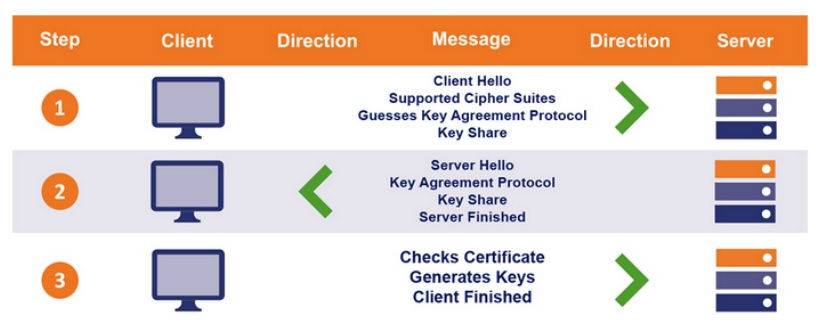
\includegraphics[width=0.8\textwidth]{img/OB-12_2.jpg}
	\end{itemize}
\end{itemize}

\subsubsection*{SSH}
\begin{itemize}
	\item Secure Shell Protocol
	\item TCP port 22
	\item transportní vrstva --- typicky běží přes TCP
	\item autentikační vrstva --- řeší autentikaci uživatele a šifrovací algoritmy, řeší autentizaci serveru
	\item spojovací vrstva --- koncept kanálů a služeb , více současných obousměrných kanálů
	\item typy kanálů --- shell, direct-tcpip (přeposílání od klienta na server), forwarded-tcpip (přeposílání ze serveru klientovi)
	\item SSH Handshake
	\begin{itemize}
		\item Diffie-Hellman výměna klíčů
		\item server klientovi posílá jak jeho vygenerované číslo $Y_b$, tak certifikát/klíč a podepsaný hash zprávy
		\item následně se vypočítá 6 kryptografických hodnot: (IV, šifrovací klíč, integritní klíč) jak pro klienta tak pro server
	\end{itemize}
\end{itemize}